\documentclass[11pt]{article}
\usepackage{amsmath,amsthm}
\usepackage{tikz}
\usetikzlibrary{positioning, shapes.misc}
\usepackage{tikz}
\usetikzlibrary{arrows,backgrounds,calc,fit,decorations.pathreplacing,decorations.markings,shapes.geometric}
\tikzset{every fit/.append style=text badly centered}

\begin{document}

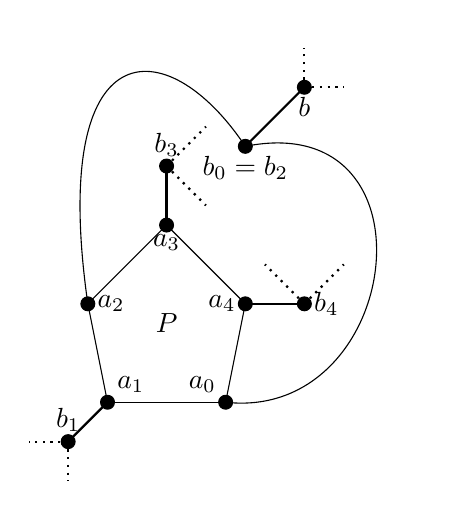
\begin{tikzpicture}[scale=0.5]
  \node at (0,0.5) {$P$};
  \filldraw [black] (1.5,-1.5) circle (5pt);
  \node[above left] at (1.5,-1.5) {$a_0$};
  \filldraw [black] (-1.5,-1.5) circle (5pt);
  \node[above right] at (-1.5,-1.5) {$a_1$};
  \filldraw [black] (-2,1) circle (5pt);
  \node[right] at (-2,1) {$a_2$};
  \filldraw [black] (2,1) circle (5pt);
  \node[left] at (2,1) {$a_4$};
  \filldraw [black] (0,3) circle (5pt);
  \node[below] at (0,3) {$a_3$};
  \filldraw [black] (-2.5,-2.5) circle (5pt);
  \node[above] at (-2.5,-2.5) {$b_1$};
  \filldraw [black] (3.5,1) circle (5pt);
  \node[right] at (3.5,1) {$b_4$};
  \filldraw [black] (0,4.5) circle (5pt);
  \node[above] at (0,4.5) {$b_3$};
  \filldraw [black] (2,5) circle (5pt);
  \node[below] at (2,5) {$b_0=b_2$};
  \filldraw [black] (3.5,6.5) circle (5pt);
  \node[below] at (3.5,6.5) {$b$};
  \draw (1.5,-1.5) -- (-1.5,-1.5);
  \draw (-1.5, -1.5) -- (-2,1);
  \draw (-2,1) -- (0,3);
  \draw (0,3) -- (2,1);
  \draw (2,1) -- (1.5,-1.5);
  \draw[thick] (-1.5,-1.5) -- (-2.5,-2.5);
  \draw[thick] (0,3) -- (0,4.5);
  \draw[thick] (2,1) -- (3.5,1);
  \draw (-2,1) .. controls (-3,8) and (0,8) .. (2,5);
  \draw (1.5,-1.5) .. controls (6,-2) and (7,6) .. (2,5);
  
  \draw[thick] (2,5) -- (3.5,6.5);
  \draw[thick, dotted] (0,4.5) -- (1,5.5);
  \draw[thick, dotted] (0,4.5) -- (1,3.5);
  \draw[thick, dotted] (3.5,1) -- (2.5,2);
  \draw[thick, dotted] (3.5,1) -- (4.5,2);
  \draw[thick, dotted] (-2.5,-2.5) -- (-3.5,-2.5);
  \draw[thick, dotted] (-2.5,-2.5) -- (-2.5,-3.5);
  \draw[thick, dotted] (3.5,6.5) -- (3.5,7.5);
  \draw[thick, dotted] (3.5,6.5) -- (4.5,6.5);
  \end{tikzpicture}

\end{document}